\documentclass{article}

\usepackage{arxiv}

\usepackage[utf8]{inputenc} % allow utf-8 input
\usepackage[T1]{fontenc}    % use 8-bit T1 fonts
\usepackage{lmodern}        % https://github.com/rstudio/rticles/issues/343
\usepackage{hyperref}       % hyperlinks
\usepackage{url}            % simple URL typesetting
\usepackage{booktabs}       % professional-quality tables
\usepackage{amsfonts}       % blackboard math symbols
\usepackage{nicefrac}       % compact symbols for 1/2, etc.
\usepackage{microtype}      % microtypography
\usepackage{graphicx}

\title{Functional traits complicate the picture of temporal biodiversity
change in bird and mammal communities}

\author{
  }


% tightlist command for lists without linebreak
\providecommand{\tightlist}{%
  \setlength{\itemsep}{0pt}\setlength{\parskip}{0pt}}


% Pandoc citation processing
\newlength{\cslhangindent}
\setlength{\cslhangindent}{1.5em}
\newlength{\csllabelwidth}
\setlength{\csllabelwidth}{3em}
\newlength{\cslentryspacingunit} % times entry-spacing
\setlength{\cslentryspacingunit}{\parskip}
% for Pandoc 2.8 to 2.10.1
\newenvironment{cslreferences}%
  {}%
  {\par}
% For Pandoc 2.11+
\newenvironment{CSLReferences}[2] % #1 hanging-ident, #2 entry spacing
 {% don't indent paragraphs
  \setlength{\parindent}{0pt}
  % turn on hanging indent if param 1 is 1
  \ifodd #1
  \let\oldpar\par
  \def\par{\hangindent=\cslhangindent\oldpar}
  \fi
  % set entry spacing
  \setlength{\parskip}{#2\cslentryspacingunit}
 }%
 {}
\usepackage{calc}
\newcommand{\CSLBlock}[1]{#1\hfill\break}
\newcommand{\CSLLeftMargin}[1]{\parbox[t]{\csllabelwidth}{#1}}
\newcommand{\CSLRightInline}[1]{\parbox[t]{\linewidth - \csllabelwidth}{#1}\break}
\newcommand{\CSLIndent}[1]{\hspace{\cslhangindent}#1}

\usepackage{lineno}
\linenumbers
\usepackage{booktabs}
\usepackage{longtable}
\usepackage{array}
\usepackage{multirow}
\usepackage{wrapfig}
\usepackage{float}
\usepackage{colortbl}
\usepackage{pdflscape}
\usepackage{tabu}
\usepackage{threeparttable}
\usepackage{threeparttablex}
\usepackage[normalem]{ulem}
\usepackage{makecell}
\usepackage{xcolor}
\begin{document}
\maketitle


\begin{abstract}
Aim: Despite unprecedented environmental change due to anthropogenic
pressure, recent work has found increasing species turnover but no
overall trend in species diversity through time at the local scale.
Functional diversity provides a potentially powerful alternative
approach for understanding community composition by linking shifts in
species identity to mechanisms of ecosystem processes. Here we present
the first multi-taxa, multi-system analysis of functional change through
time.

Location: Global, with a North American focus

Time period: 1923-2014

Major taxa studied: Mammals, Birds

Methods: We paired thousands of bird and mammal assemblage time series
from the BioTIME database with existing trait data representative of a
species' functional role to reconstruct time series of functional
diversity metrics. Using generalized linear mixed models, we estimated
general trends in those metrics and trends for individual studies.

Results: We found no overall trend in any functional diversity metric,
despite data replicating species-based patterns of constant richness
with increasing turnover. The lack of trend held even after correcting
for changes in species richness. At the study-level, there were also a
substantial number of time series exhibiting no species or functional
change, however most studies showed a shift in a species or functional
metric.

Main Conclusions: General trends indicate that on the aggregate one type
of functional shift is not more prevalant than the other across many
taxa, biomes, and realms. At the study-level, we identified four
prevailing scenarios of species and functional change, which showed
links to the duration of the observation window. With no one prevailing
scenario of change, it will be critical to link change scenarios to
drivers of change, particularly to identify communities with capacity to
resist drivers from those not experiencing substantial pressure from a
driver.
\end{abstract}

\keywords{
    biodiversity change
   \and
    functional traits
   \and
    global change
   \and
    time series
  }

\hypertarget{introduction}{%
\section{Introduction}\label{introduction}}

Ecological communities are experiencing unprecedented change as a result
of anthropogenic pressures such as climate change, land use change, and
invasive species. Impacts of these pressures are well documented at a
global scale by an accelerating global extinction rate (1), and
fundamental changes in some of the most well-studied systems (e.g.~coral
bleaching, 2). At the local scale however, species diversity tells a
different story. Recent syntheses of local trends in biodiversity over
time have found no net change in local species diversity despite ongoing
turnover (3--6) and evidence of significant shifts in community
composition underlying consistent species richness (7--9). While
communities are clearly changing, our most common species-based
approaches do not fully capture the nature of that change.

The meaning of general trends derived from limited data, and their
relevance for conservation, is a topic of on going debate. Global
analyses have been heavily criticized for geographic biases, lack of
data in the most heavily impacted areas, and exclusion of individual
studies' ecological context (10--12). Many of these criticisms reflect
limitations of ecological data on the whole,
\textcolor{blue}{leading to a call for additional data not only to fill geographic and temporal gaps, but to flesh out key characteristics of communities}
(13, 14).

Functional diversity offers a potentially powerful addition to
species-based approaches for detecting and describing community change
by providing a mechanistic link between species' response to
environmental change (\emph{response traits}) and the processes they
perform (\emph{effect traits}) (15--17). By describing the functional
trait space, functional diversity metrics capture the disproportionate
impact of losses or gains of functionally unique species. Functional
diversity metrics
\textcolor{blue}{may therefore illuminate joint responses from functionally similar species or communities undetectible by looking at species identity alone.}

\textcolor{blue}{The expectation for functional change across communities is not obvious from past work, and may or may not follow taxonomic trends}
(13). While functional loss is frequently cited as one of the most
pressing concerns of the anthropocene (18--20),
\textcolor{blue}{functional diversity may be maintained even when species are lost from a community}
(21, 22). Forecasts of functional loss range from negligible (23) to
dire (24, 25). And while some observed trends show significant
functional loss (26) others document no loss even in some of the most
heavily impacted communities (27--29). On paleoecological time scales,
functional composition shows mixed responses to environmental change and
extinction events (30, 31), with significant impacts of species
extinctions on functional diversity in some taxa and not others (32).
For some time periods, functional structure appears to be maintained for
substantial portions of geological time (33).
\textcolor{blue}{Contemporary, broad-scale examinations of functional change are limited to only a few taxa-focused studies, but show for example functional richness increases for both North American birds [@barnagaud2017; @jarzyna2016] and ray-finned fishes, sharks, and rays}
(34).

Here we
\textcolor{blue}{leverage ongoing efforts to assemble functional trait data and recent computational advances to}
perform the first multi-taxa, multi-realm assessment of functional
diversity change through time. We focus on mammal and bird species as a
significant subset of the world's biodiversity heavily impacted by
anthropogenic change. While examining trends in plants, invertebrates,
and other vertebrate species is of equal interest, trait data for those
taxa raise additional challenges such as limited and biased species
coverage (35), a lack of accepted species-level means, and differences
in the types of traits collected. To ensure comparability across taxa in
trait type and data quality we therefore focus on mammals and birds.
Traits were intentionally selected to be representative of a species'
Eltonian niche, thereby summarizing the functional role they play in the
community (36). An initial assessment of amphibian trends is included in
the supplement, but excluded from general trend assessment here due to
limited geographic coverage.

We assess thousands of mammal and bird functional diversity time series
to determine whether or not
\textcolor{blue}{the addition of functional trait data gives a clarifying picture of biodiversity change across communities. Rather than testing specific hypotheses of change we present a few areas of change consensus across communities, and even more scenarios where the relationship between functional and species change are unexplained and warrant further theoretical and experimental examination. We present results at three different levels: general trends across communities, trends for communities with similar characteristics (taxa, biome, realm, protection status), and trends for individual studies.}

\hypertarget{material-and-methods}{%
\section{Material and Methods}\label{material-and-methods}}

\hypertarget{data}{%
\subsection{Data}\label{data}}

We obtained mammal and bird time series from the BioTIME database, a
global repository of high-quality assemblage time series. All studies
included in the database follow consistent sampling protocols and
represent full assemblages rather than populations of single species
(31). All time series include abundance of observed species. Following
best practices for the database (37), studies with multiple sample
locations were split into individual time series following a
standardized spatial scale. Scale was set by a global grid with cell
size determined based on the sample extent of studies with only a single
location (see 31 for details on how sample extents were defined), with
the area of each cell set to one standard deviation away from the mean
of the single extent locations. All samples from a study within a single
cell were considered to be a single time series, and species abundances
were combined for all samples.

We used trait data from the Elton Trait Database, which consists of
species-level means for traits that represent species' multifaceted role
in the community (36). Traits include: body mass, diet, active diel
period, nocturnality, forest foraging strata, pelagic use. Multiple
traits (i.e.~diet, foraging strata, activity seasonality, active diel
period) were broken down into percentage or binary use for each level.

In order to ensure taxonomic consistency across datasets, BioTIME
species were paired with trait data based on their species identifier
from the Integrated Taxonomic Information System database (retrieved
09-15-2020 from the on-line database,
\url{https://doi.org/10.5066/F7KH0KBK}), obtained through the
\texttt{taxadb} R package (38, 39). If more than one species in the
assemblage data resolved to the same identifier, observations were
considered the same species. For trait data, traits for all species of
the same identifier were averaged. Only studies for which at least 75\%
of species had trait data were included. In order to have a sufficient
number of species to calculate functional diversity metrics, years with
fewer than 5 species observed were also excluded. Sensitivity analyses
were conducted for the trait coverage threshold and the duration of
included time series.

Many studies had a variable number of samples within years. To account
for this inconsistency in sampling effort we used sample-based
rarefaction by bootstrap resampling within years for each time series
based on the smallest number of samples in a year for that time series.

Our final dataset included 2,432 time series from 50 studies in 21
countries and 12 biomes and 6 different traits (Fig \ref{fig:taxaMap}).
Data came from both terrestrial and marine realms and five climates
(Global, Polar/Temperate, Temperate, Temperate/Tropical, Tropical). The
earliest sample was in 1923 and the most recent was in 2014.
\textcolor{blue}{While it is not possible with this data to directly assess the level of human impact occurring for each study, we include binary protection status as a coarse indicator of impact level. However, protected areas were almost exclusively from temperate terrestrial studies (with one tropical study), so results are confounded by multiple other study characteristics.}
For a full breakdown of studies and their characteristics, see the
supplement. Our final dataset reflects many of the data biases that make
global synthesis work challenging, including geographic bias, a bias
away from areas currently under the greatest threat, and a bias towards
shorter time series. We address these shortcomings and their potential
impact on our results in the discussion.

\begin{figure}
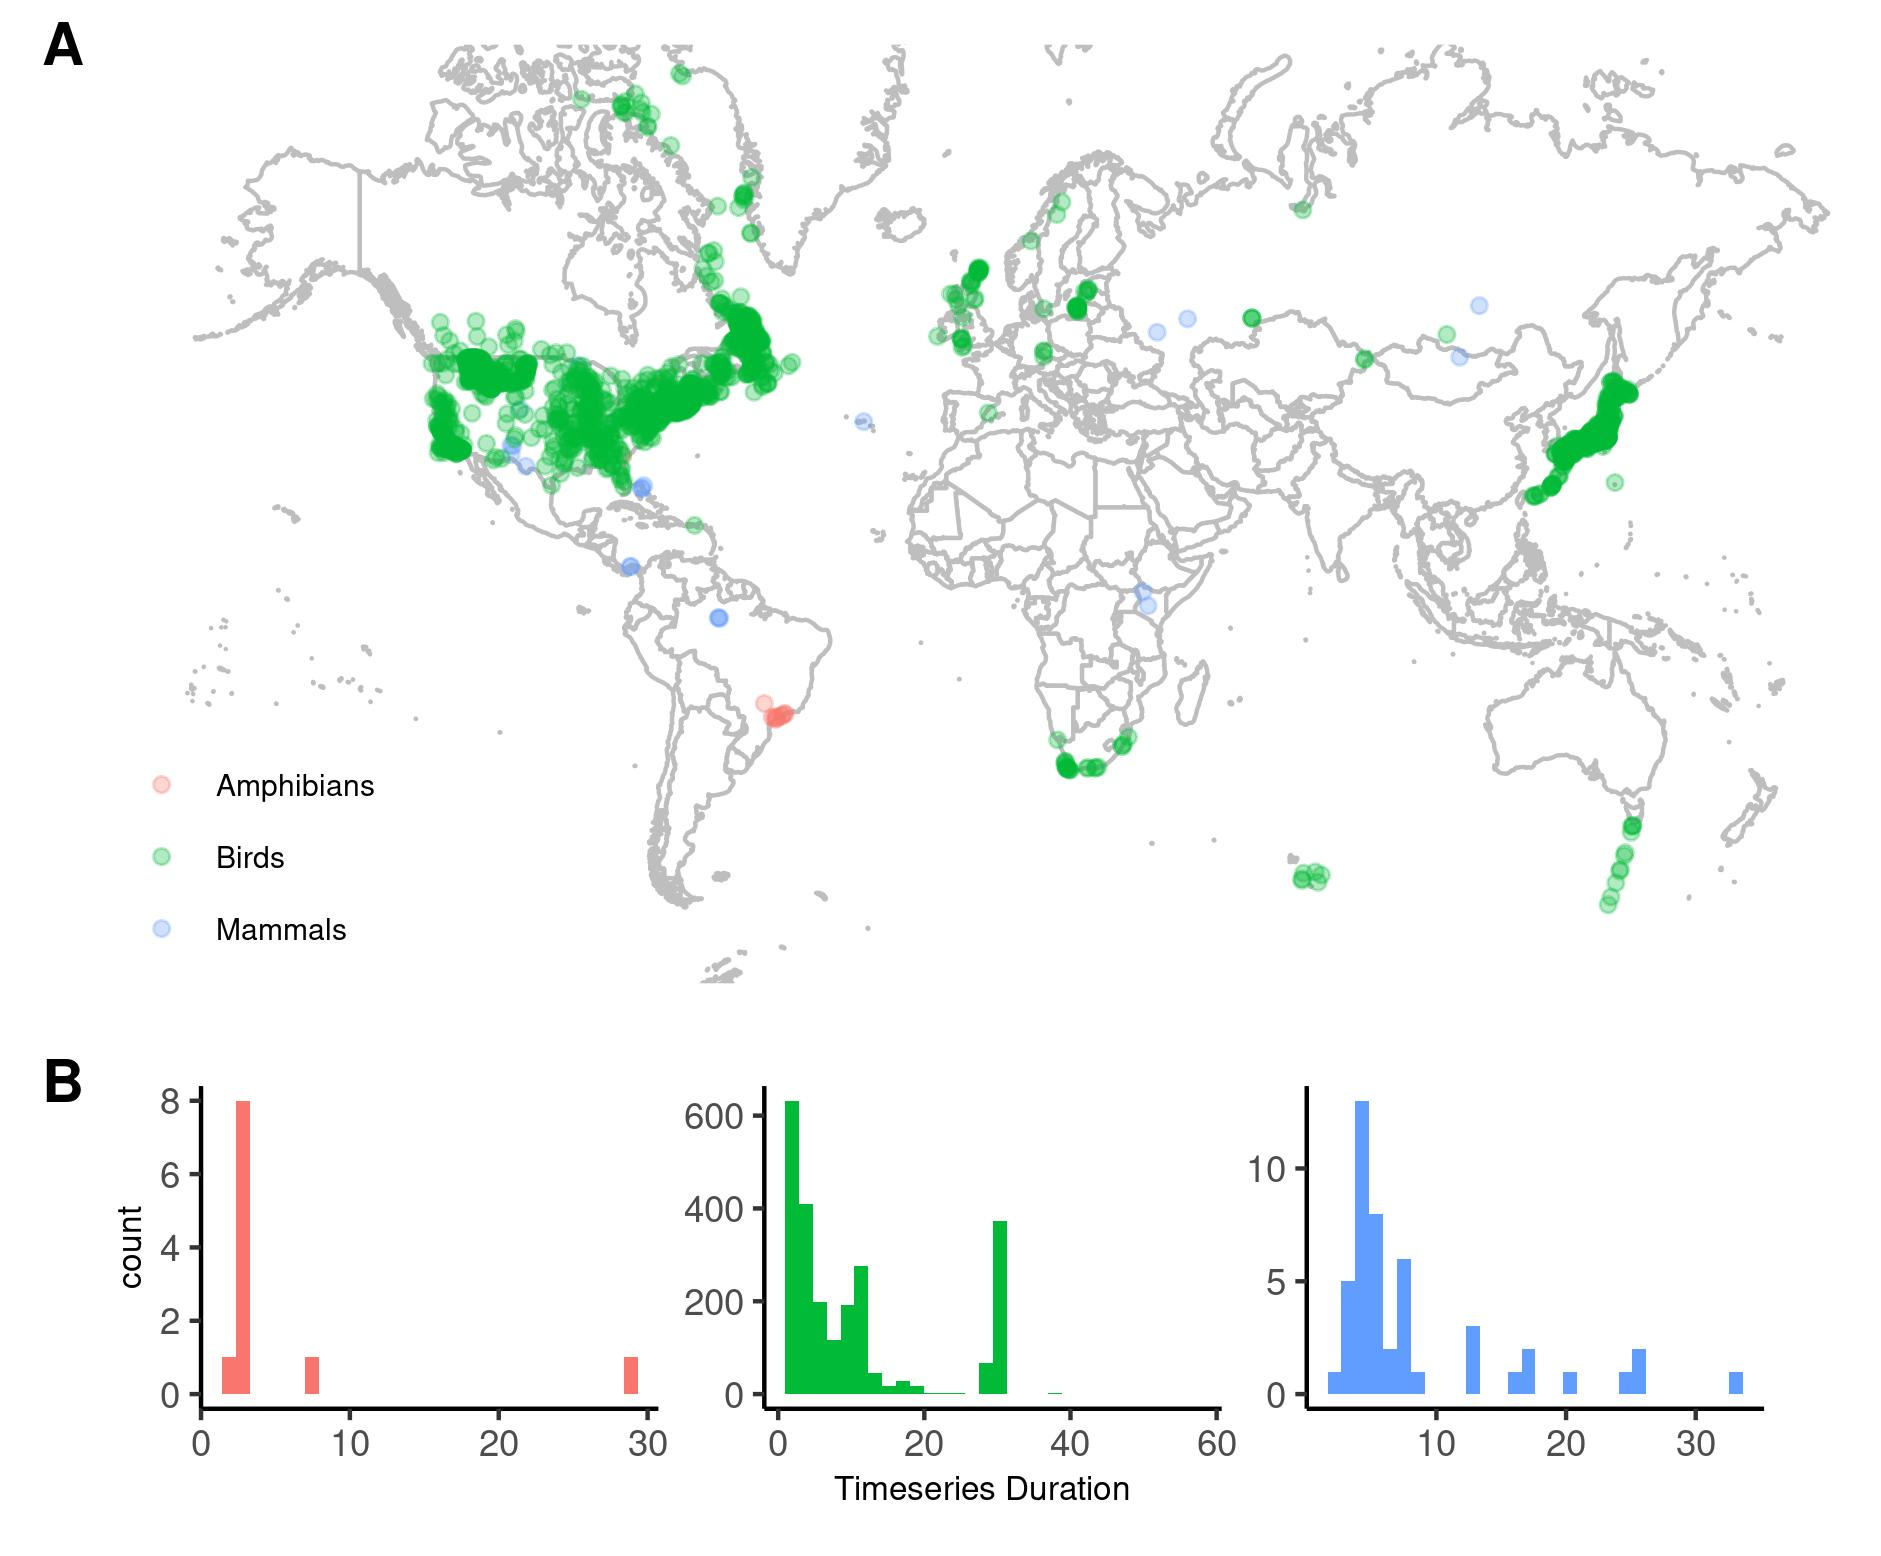
\includegraphics[width=\textwidth]{../../figures/study_map_hist} \caption{A) Map of time series locations with points colored by taxa, and B) histograms of time series duration broken down by taxa.}\label{fig:taxaMap}
\end{figure}

\hypertarget{diversity-metrics}{%
\subsection{Diversity Metrics}\label{diversity-metrics}}

We calculated yearly metrics of functional and species diversity for
each time series. Species-based metrics include species richness
(\emph{S}) and Jaccard similarity (\emph{J}) as a measure of turnover.
Jaccard similarity was calculated relative to the first observed year
for a time series. A negative trend in \emph{J} would therefore indicate
increasing turnover. We did not impose a correction for unobserved
species as non-parametric estimators do not assign species identities to
corrected richness values, and therefore could not be propagated to the
functional diversity metrics.

Functional diversity metrics were calculated using the \emph{dbFD}
function from the \emph{FD} R package (40). Here we report functional
richness (\emph{FRic}), functional evenness (\emph{FEve}), and
functional divergence (\emph{FDiv}) which together describe three
complementary characteristics of the functional space (41, 42).
\emph{FRic} assesses the volume of the trait space occupied by species
in the community, with higher values indicating communities with species
of more extreme trait values. \emph{FEve} describes how species are
distributed across the trait space and how abundance is distributed
across species. Higher values of \emph{FEve} indicate more even spacing
of species in the trait space and individuals across species.
\emph{FDiv} measures the degree to which species and their abundances
maximize differences in the functional space. Higher values of
\emph{FDiv} therefore correspond to communities where many highly
abundant species are on the edges of the trait space. We also calculated
the community-weighted mean (\emph{CWM}) of included traits to examine
shifts in the distribution of each trait.
\textcolor{blue}{Hereafter we refer to results for functional diversity metrics (FRic, FEve, FDiv) and composition metrics (trait CWM's).}

All available trait data for each study were included in functional
diversity calculations with the exception of traits that were the same
value for all observed species in the study. For variables with multiple
levels each level was included as a separate trait axis. Continuous
traits were z-score scaled to give each trait equal weight in the trait
space (43, 44).
\textcolor{blue}{Before calculating diversity metrics, dbFD reduces the dimensionality of the trait space by performing PCoA. We limited the number of included PCoA axes to}
the maximum number of traits that fulfills the criteria \(s >= 2^t\),
where \(s\) is the number of species and \emph{t} is the number of
traits. This restriction allows for enough axes to capture the trait
space while maintaining computational feasibility (45). Metrics
incorporated weighting based on species abundance.

\hypertarget{null-models}{%
\subsection{Null Models}\label{null-models}}

To assess functional change independent of species richness we
calculated the standardized effect size (SES) for each of the three
functional diversity metrics (\emph{FRic}, \emph{FEve}, \emph{FDiv})
from null estimates (46). Null model corrections allow us to assess the
degree to which the observed functional diversity metric deviates from
the value expected by chance in a randomly assembled community. Null
estimates were calculated for each rarefied sample by randomly sampling
species from the species pool for each year and randomly assigning
observed abundances to species. `
\textcolor{blue}{Species pools were unique for each time series and included all species observed over the course of sampling, therefore accounting for geographic restrictions in species availability}.
This process was repeated 500 times to get an estimate and standard
deviation of the null expectation for the metric for each rarefaction
sample for that time series. We used these values to calculate SES using
the following formula:
\(SES = [F_{obs} - mean_{(F_{null})}]/SD_{(F_{null})}\). We then
calculated the median SES estimate for each metric from all the
rarefaction samples for a time series. SES estimates can be interpreted
as how much of the functional characteristic (richness, evenness,
divergence) was observed beyond what was expected by chance for a
community of that species richness.

\hypertarget{analysis}{%
\subsection{Analysis}\label{analysis}}

We estimated general trends
\textcolor{blue}{across bird and mammals communities} for each diversity
metric using a linear mixed effects model with a random slope and
intercept for each study and each time series nested within the study.
We fit 18 individual \emph{CWM} models. All time series with data for a
given trait were included in the corresponding \emph{CWM} model. We
estimated study level trends using individual linear models. For studies
with more than one times series we fit a random slope and intercept for
time series. Some study-level models could not be fit for five studies
for at least one metric due to data limitations, but those studies were
still included in the general models. They represented 12 of 1350
study-level models fit for each metric. For further details see the
supplement. Where appropriate, response variables were \(log\) or
\(log(x+1)\) transformed to better fit model assumptions of residual
normality.

To test for trends within and between different levels of taxa, biome,
realm, and protection status we fit separate models with each of those
factors added as a predictor interacting with time to the original model
structure. We estimated within-level slopes and calculated between-level
contrasts using the \emph{emmeans} package (v1.8.2, 47). We assessed the
impact of time series duration and start year on study-level trends
using linear models with duration and start year as predictors. All
models in our analysis were fit using the \emph{lme4} (v1.1-30) package
in R (v4.2.3) and p-values were calculated by Satterthwaite's degrees of
freedom method using the \emph{lmerTest} (v3.1-3) package with a
significance level of \(\alpha = 0.05\) (48--50).

\hypertarget{results}{%
\section{Results}\label{results}}

We found no significant overall trend in species richness or functional
diversity metrics (observed or \textcolor{blue}{corrected}) (Fig
\ref{fig:timeseriesPlot}). We did find a significant overall decrease in
Jaccard similarity, indicating accumulating changes in species
composition. Non-significant overall trends indicate that although some
studies experience increasing or decreasing trends, the average trend
across studies was plausibly 0 (Table \ref{tab:resultsTab}).
\textcolor{blue}{Within-group} trends for different taxa, biomes,
realms, or protection statuses were also non-significant for richness
and functional diversity metrics, with the exception of a significantly
increasing trend for functional evenness of global studies
(characterized by having samples on multiple continents), and a
significantly decreasing functional richness slope for
temperate/tropical studies and mammal studies. However, trends were not
exhibited for the \textcolor{blue}{corrected} metric indicating that
differences \textcolor{blue}{in functional diversity metrics} were
largely due to changes in species richness. Further, with only two
global studies, the trend should not be considered truly general. The
general trends for \emph{CWM} models were similarly not significant,
with a significant positive trend for only percentage of fish in diet
composition.

\begin{figure}
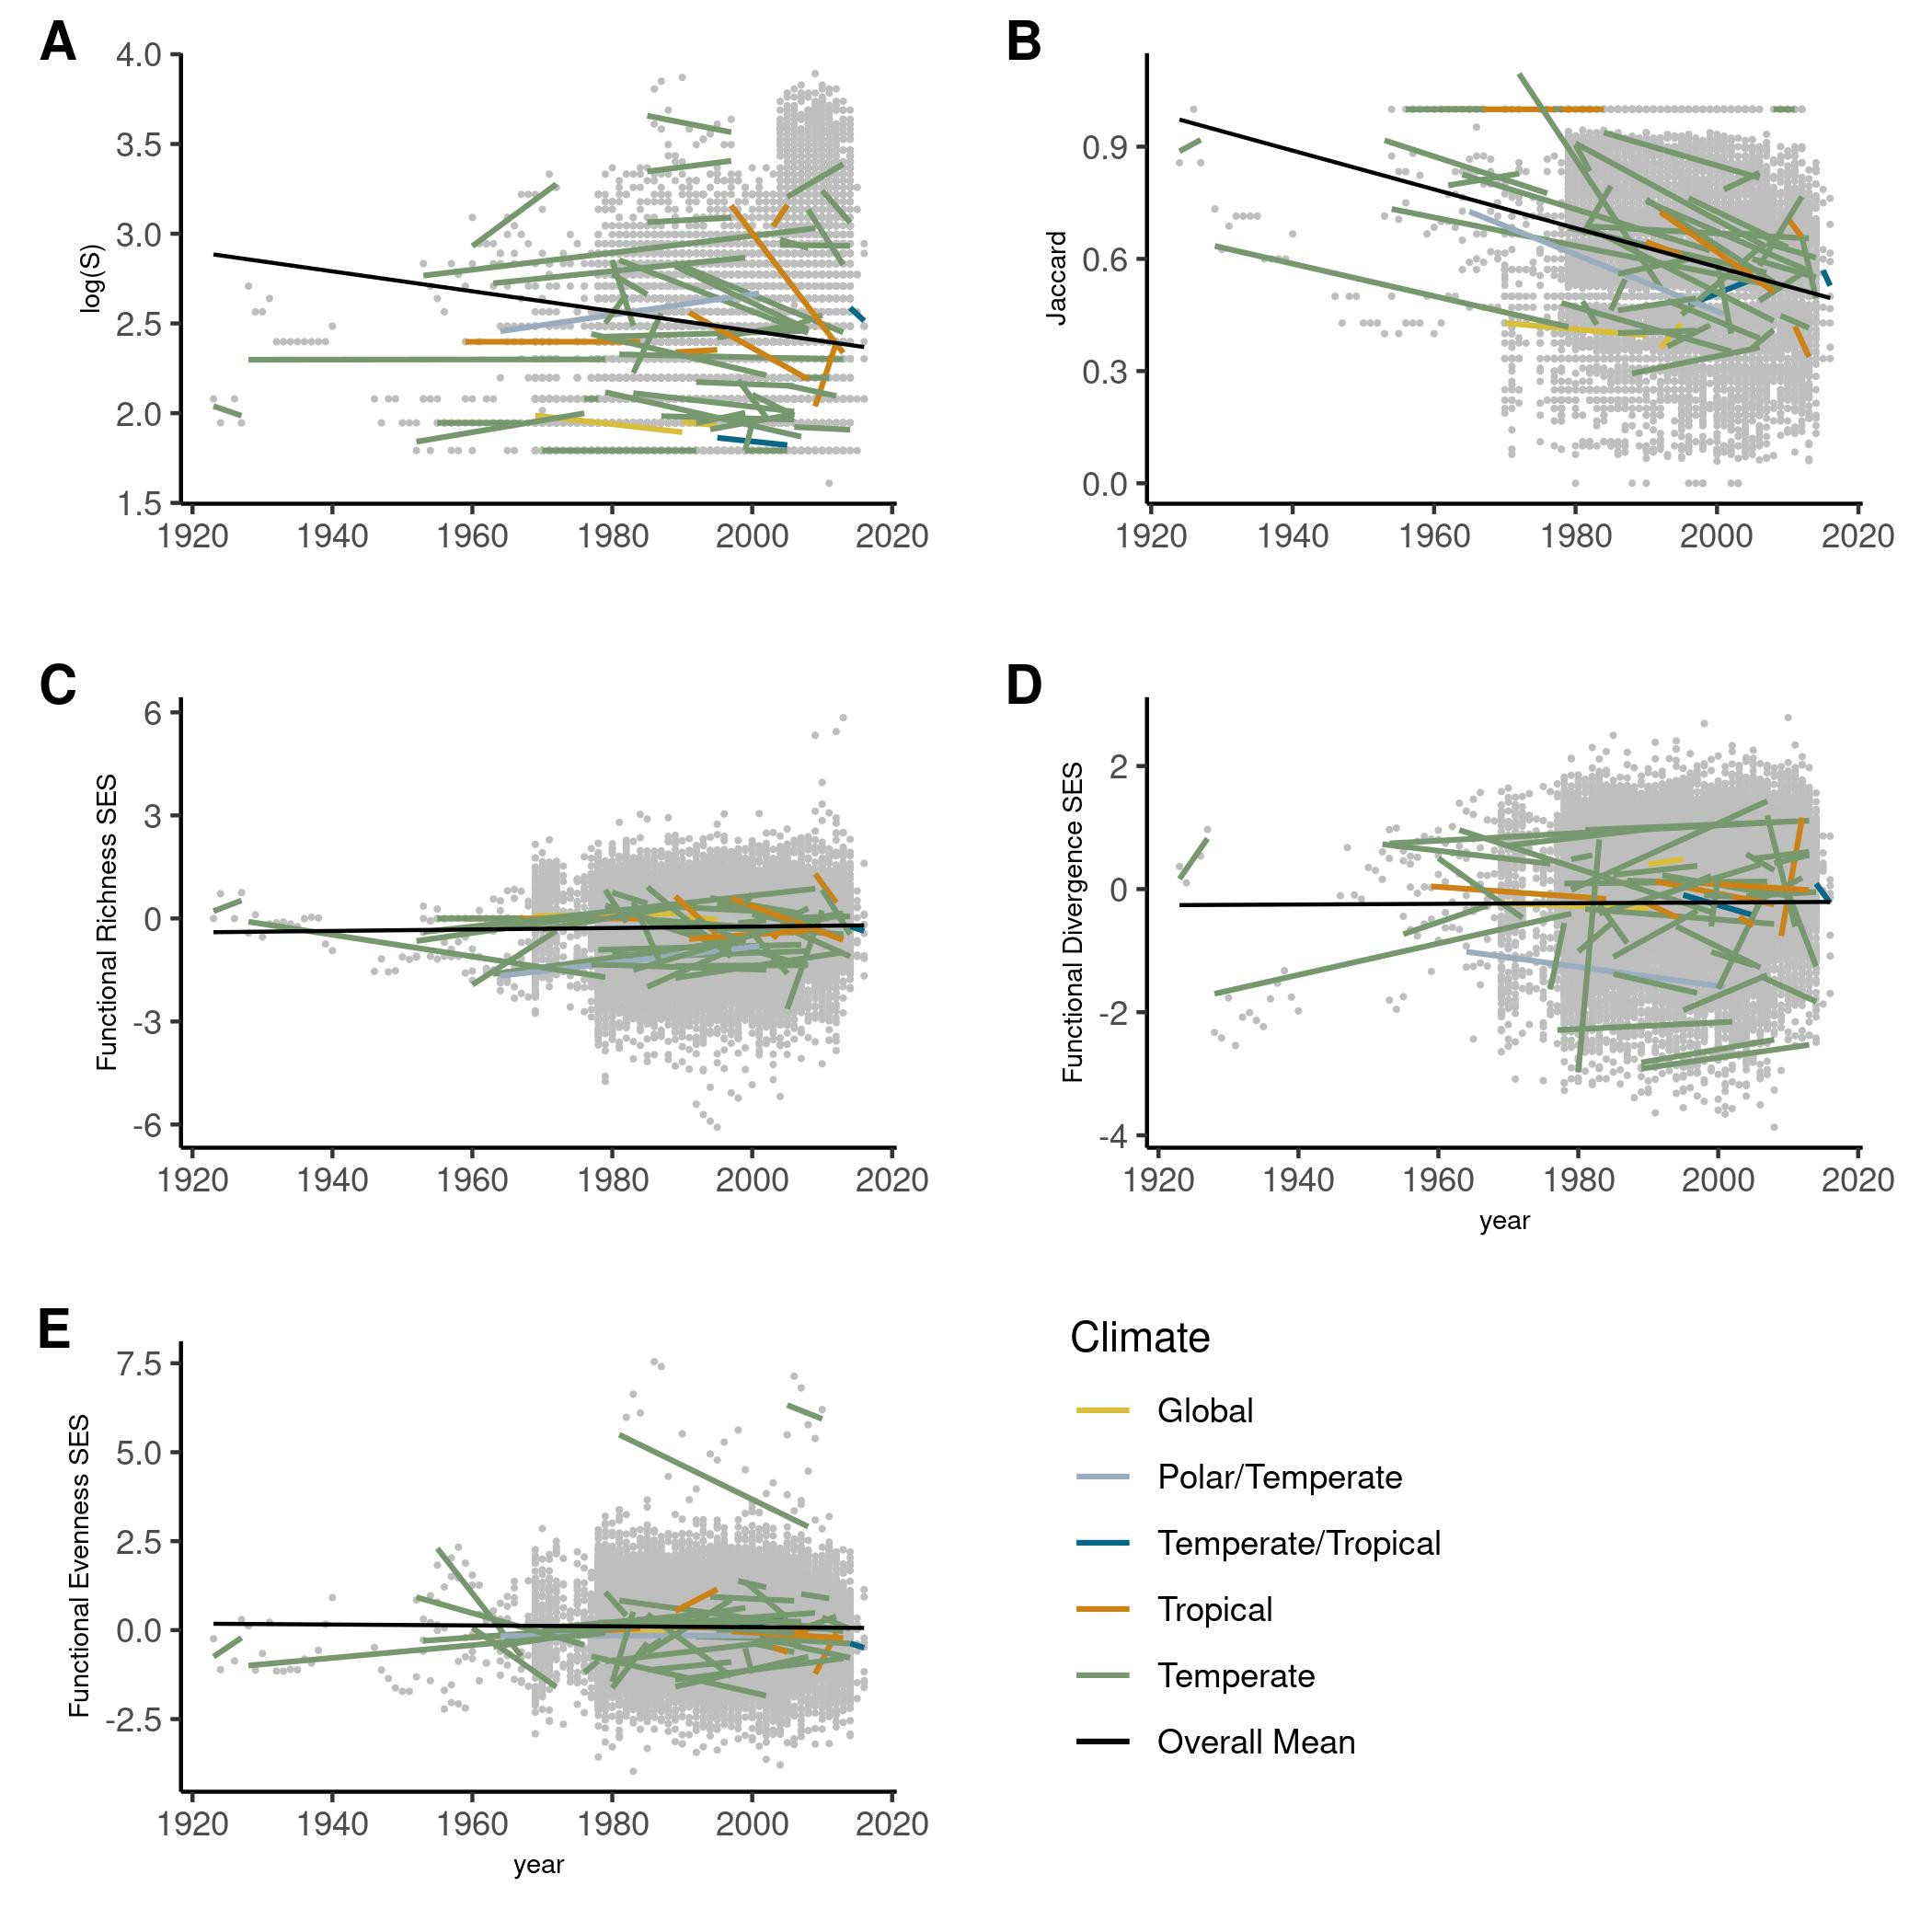
\includegraphics[width=\textwidth]{../../figures/3met_long} \caption{Plots of time series-level trends with line color corresponding to climatic region, with data points in grey and the overall metric mean in black for A) log species richness, B) Jaccard similarity, C) Functional Richness SES, D) Functional Divergence SES, and E) Functional Evenness SES}\label{fig:timeseriesPlot}
\end{figure}

We did find significant differences between taxa, realms, and climate
for Jaccard similarity and some of the \emph{CWM's}. For example, while
Jaccard similarity was decreasing in the general trend and there were
significant within group slopes for Mammals, Birds, and Terrestrial
communities, there was no significant slope for the marine realm,
indicating that the general trend is mostly driven by turnover in
terrestrial communities. We also found a significant decrease in Jaccard
similarity in unprotected areas only, with no trend for protected areas.
For bird communities, we also found within group trends and between
group differences for trends in foraging behavior. We found a
significant increasing trend in utilization of the canopy in Tropical
communities that was significantly different from the trends for
Polar/Temperate and Temperate communities. There was a significant
decrease in utilization of the understory for Terrestrial communities
and significant increase in foraging below the water surface for global
studies (but see the previous limitations of Global data). There was
also a significant positive slope for \emph{CWM} body mass for the
single Temperate/Tropical study (with three time series) which were
marine mammal communities.

We found significant dietary shifts across communities, with a
significant increase in fruit consumption in Terrestrial communities and
a significant decrease in nectar consumption in Tropical communities, a
trend significantly different than that for Terrestrial communities.
There was a significant increase in seed consumption in bird species,
which was significantly different from the trend for Mammal communities.
There was a significant increase in fish consumption for the two Global
studies. Vertebrate consumption significantly decreased for Marine
studies and for studies of Global and Tropical communities.
\textcolor{blue}{There was also a significant increase in fish and fruit consumption for unprotected areas, but not protected.}

At the study level, 15 of 50 studies exhibited a significant trend in
species richness and 11 exhibited significant turnover. For observed
functional metrics, 25 of 50 studies exhibited a trend in a least one
metric, and 15 of 50 studies exhibited a significant trend for at least
one \textcolor{blue}{corrected} metric (Table \ref{tab:trendTab}). In
general, there were more significant trends for uncorrected metrics,
with some disappearing after correction, indicating that those trends
were likely due to changes in the number of species. Hypothesis testing
for study-level trends is likely affected by multiple testing issues and
some trends identified as significant are therefore potentially
spurious. Rather than interpreting changes in specific studies, we
present these results as a general picture of the kinds of trends
experienced by communities.

Study-level slopes for functional diversity metrics were significantly
related to start year of the time series for Jaccard similarity and
functional evenness, both of which had significantly more negative
slopes with more recent start year. No functional diversity metrics were
significantly related to the start year of the time series.

We assessed the sensitivity of general trend results to major data
processing decision by rerunning models with increasingly conservative
subsets of the data. After excluding time series with less than two,
three, and four year durations, we found that the general trend for
increase in CWM aerial foraging disappeared, but two other trends in
CWM's appeared. After excluding time series two years long, a general
trend appeared for increased CWM use of the forest canopy, and decreased
CWM of seed consumption. These two trends remained as increasingly
shorter time series were excluded suggesting the increase in aerial
foraging was an erroneous finding while the other two trends were more
robust. Percentage of species in a community with trait data did not
appear to have an affect on general trend results, as general trends
were unchanged with increasing cut offs for percentage of species with
trait data. A complete list of models run in the sensitivity analysis
and their results can be found in the supplement.

\hypertarget{discussion}{%
\section{Discussion}\label{discussion}}

Our study represents the largest broad-scale multi-taxa assessment of
functional change through time to date, giving a first look at aggregate
and local trends in functional diversity in mammal and bird communities.
\textcolor{blue}{Our results show that the addition of functional traits illuminates a few consistent functional trends across communities, but largely complicates rather that clarifies the story of biodiversity change. While the characteristics of species clearly matter, instead of unifying the nature of communities' change, they more often distinguish them. In general, we found a few areas of consensus for models where communities were aggregated (general trends, trends by taxa, biome, realm, protection status), and vast heterogeneity for study-level models.}

\hypertarget{evidence-of-consensus}{%
\subsubsection{Evidence of consensus}\label{evidence-of-consensus}}

\textcolor{blue}{The most stark area of consensus was the lack of general trend aggregating across communities.}
We did not detect an overall trend in any functional diversity metrics.
As with previous species-based syntheses, we also found no overall trend
in species richness accompanied by increasing turnover through time
(31), indicating that non-significant trends in functional metrics are
consistent with similar well-documented species derived trends. We found
no trend in functional change for almost all realms, biomes, and
taxonomic groups.
\textcolor{blue}{The one exception was a consensus trend indicating}
functional richness loss for mammal studies. These results are
consistent with multiple studies linking anthropogenic drivers to loss
of functional diversity in mammal communities (51--53).

Despite a lack of general trends in functional diversity metrics, we did
find evidence of compositional shifts in the trait space with multiple
\texttt{significant} trends in \emph{CWM}'s for studies coming from the
same taxa, realms, climates, or protection statuses,
\texttt{indicating\ areas\ of\ consensus\ change\ across\ communities}.
Some of those trends are consistent with existing work in those
contexts. For example, the decrease in insect consumption for tropical
communities reflects well documented declines in tropical insectivorous
birds (54). Reduction in utilization of understory foraging for
terrestrial communities could be the result of disturbance like human
recreation or increased predation from introduced species. Other shifts
in diet for both Birds and Mammals, including increasing fruit, seed,
and vertebrate consumption and decreasing seed consumption in some
climates point to important areas for further exploration.

\hypertarget{study-heterogeneity}{%
\subsubsection{Study heterogeneity}\label{study-heterogeneity}}

\textcolor{blue}{At the study-level, our results run contrary to our hope for a clearer picture of biodiversity change through a functional lens. The lack of general trend in functional diversity metrics belies a huge range of positive and negative trends at the study-level. In order to simplify discussion, we will talk about the implications for ecosystem process and vulnerability for communities grouped by their concurrent change in functional diversity metrics, species richness and turnover split into positive, negative or no trend. While there are over 150 possible combinations of change direction (or no change) in the 5 metrics, we discuss here the six scenarios that occurred in more than one study: no change, species loss or gain only, loss of functional evenness, richness loss with species turnover, and increase in species and functional richness accompanied by significant turnover. We focus on these scenarios to combat potential spurious results due to multiple testing, as it is unlikely all observations of the same scenario are due to false positives. We include a break down of the number of studies in each scenario to illustrate relative number of studies in each group, but emphasize that the absolute number is likely impacted by multiple testing.}

The majority group of studies exhibited no trend in any species or
functional diversity metric. Contrary to the expectation due to
anthropogenic and global change stressors, these communities do not show
significant changes over the course of the observation window. Studies
in this group span the distribution of study durations excluding only
the very longest running studies, with the longest no change time series
lasting 23 years. They also included both bird and mammal studies and
only four were located in protected areas, indicating that the lack of
trend is not restricted to a specific ecological context or those
communities most insulated from human impact.

The lack of trend could be the result of multiple possible scenarios.
First, these may be communities resisting perturbations or simply not
experiencing significant perturbations. Given the studies in this group
come from all possible taxa, realms, climates, and protection statuses,
evidence points to communities resisting perturbation, offering some
hope that there are areas of the globe where communities are fairing
well for now. Alternatively, these may be communities that have
experienced or continue to experience significant stress, but lost
species or functional diversity outside the observation window. This
could be true particularly for North American mammal communities where
trophic downgrading and megafaunal losses occurred hundreds of years ago
{[}citation{]}. Third, these communities may be experiencing directional
shifts undetectable by available data. For example, species-level trait
data does not capture intraspecific shifts in the trait space, which can
represent significant changes in overall functional composition and
impact maintenance of ecological processes {[}citation{]}.

Three of the groups fit under the broad umbrella of changes in
redundancy. By definition, if a community gains or loses species while
functional metrics are unchanged, those species represent an increase or
decrease in redundancy, so we include communities exhibiting gains or
losses in species richness with no change in functional metrics or
turnover and richness loss with significant turnover in this umbrella.
For communities exhibiting loss of redundancy (declining species
richness), ecological processes are likely being maintained, but
capacity to respond to future stressors is reduced (55). These
communities are actually fairing better than expected looking at
species-based metrics alone, but are also in a precarious position for
maintaining ecological function into the future (56). Conversely,
communities exhibiting a increase in redundancy (via an increase in
species richness) are becoming better positioned to respond to future
stressors, but are not actually expanding their functional capacity as
may be assumed by looking at species gains alone (57).

The next group of studies exhibit an increase in species richness and
functional richness with significant turnover. While these communities
are losing some species that are functionally redundant or functional
analogs of species additions, they are gaining even more species that
expand the functional space. These communities have a hopeful
trajectory, as they are improving their functional capacity and
potentially their functional redundancy, likely leading to robust future
ecological function. Notably, the studies that exhibited species
richness increases (in this group with increasing functional richness,
as well as communities without functional richness increases) were
exclusively from terrestrial, temperate (sometimes temperate/polar) bird
communities and occurred in countries where there has been a significant
investment in conservation over the last few decades (United States,
Canada, Sweden). Our results are consistent with other functional work
in these regions, showing increases in species richness and functional
diversity for North American breeding birds over the last few decades
after a period of decline(58), and loss of common, functionally general
species even as rare species are increasing in North America and Europe
(59--61).

The final group exhibits decreasing functional evenness. The empirical
link between changes in evenness and ecosystem process is the most
poorly studied of the metrics, however theory indicates that increased
evenness improves function and stability (62). If one or a few species
become largely dominant in a community, function will be the result of
only those species rather than spread out across a wealth of species
responding independently to environmental change (42, 63). Further,
there is some evidence that maintaining evenness is important for
supporting multifunctionality in communities (64). These communities are
therefore of particular concern, especially considering evidence
evenness is more sensitive to environmental change that richness (62).

While the majority of studies fell into one of the groups discussed in
detail above, 25\% of the studies exhibited some different combination
of change in metrics, underlining the vast heterogeneity of realized
change scenarios. We have an indication of the ecological
characteristics most likely to lead to some of the change types
(e.g.~temperate bird communities are gaining species and functional
richness), but most types of change are exhibited across many different
kinds of communities. Identifying key factors mediating the kind of
biodiversity change a community experiences is critical for identifying
areas of conservation concern and extrapolating results to areas where
functional trait data may not be available. While it is tempting to draw
a one to one line between the degree of human impact and loss of
functional integrity (in the form of functional redundancy and
richness), that relationship is not borne out by our rough metric of
human impact or previous taxa-specific or single community work, which
is largely mixed (26, 65--67).

\hypertarget{areas-of-incongruence}{%
\subsubsection{Areas of incongruence}\label{areas-of-incongruence}}

\textcolor{blue}{The addition of functional trait illuminated a few other key areas where a synthesis approach is incongruous with system-specific studies or expectations based on anthropegenic impacts.}
For example, mean body size is predicted to decrease as a result of
climate change impacts and megafaunal loss (68), a phenomenon which has
already been well documented empirically and experimentally in multiple
taxa (69--72). However, we found no evidence of a trend in \emph{CWM}
body size, with the exception of a single study of marine mammals in the
Bahamas which showed a significant increase.
\textcolor{blue}{While the lack of trend could be explained at least in part by data limitations such as shortened observation windows or missing intraspecific data, the fact that only one of the 41 studies for which study-level models were fit showed a change in mean body size, and in the opposite direction of the expectation, is suprising and warrants further reconciliation.}

Results for protected areas were also surprising given

\begin{itemize}
\item
  changes in diet
\item
  turnover outside protected areas, not inside ( though might be driven
  by the fact that there's generally less turnover in terrestrial and
  temperate studies) (37)
\end{itemize}

\hypertarget{policy-implications}{%
\subsection{Policy Implications}\label{policy-implications}}

While we found no over all trends in functional metrics, our results
should not be interpreted as an indication that the ongoing biodiversity
crisis is less severe than previously described, or that there is no
concern for functional change as a result of anthropogenic impact. In
fact, study-level trends indicate quite the opposite, that functional
shifts with unknown implications for ecosystem processes may be going
undetected by common species-based approaches, particularly for short
observation time windows. While the majority of studies in our dataset
did not experience a significant functional loss, a substantial body of
work links functional degradation to species losses as a result of
direct human intervention in the form of land use change and
intensification or habitat fragmentation, indicating that those studies
are simply not representative of the kinds of impacts of greatest policy
concern (67).

\hypertarget{future-work}{%
\subsection{Future Work}\label{future-work}}

We present here four prevailing scenarios of change experienced in bird
and mammal communities. While we offer a first discussion of which kinds
of change are most common and why, assessing the true global prevalence
will require continued efforts to fill data gaps, a well recognized
challenge in ecology (6, 12, 73). Still, a ``scenarios of change''
framework can provide structure for future work addressing functional
shifts, particularly as we reconcile results from broad-scale syntheses
with in-depth single system studies. It will be particularly critical to
link forms of change to individual drivers to assess which drivers may
impact species and functional diversity differently. Understanding those
links will help identify where directly measuring functional structure
instead of just species change is necessary for understand impacts on a
given system. In addition, direct links to drivers will improve our
ability to distinguish between communities experiencing no change due to
a lack of perturbation from communities with high resilience in the face
of disturbance.

Here we identify trends that are statistically significant, however they
may not necessarily be ecologically significant. While it is common to
link changes in functional metrics to changes in ecosystem processes,
those changes are less frequently discussed in terms of the size
necessary for ecological impact. The degree of change in a process
considered ecological meaningful is somewhat subjective and a function
of the system and management context, making identifying the ecological
meaning of broad-scale aggregate shifts even more challenging. It is
further hampered by the use of species-level trait data, as the traits
most closely linked to a process of interest may not be available (74).
Future trait collection that explicitly considers existing frameworks
for linking traits to processes (e.g.~the response and effect framework
15) would facilitate improved ecological interpretation of potential
functional changes.

\hypertarget{acknowledgments}{%
\section{Acknowledgments}\label{acknowledgments}}

We thank the scientists who contributed to and maintain the biodiversity
databases included in this study, including BioTIME, Amphibio, and Elton
Traits.

We thank Dr Shane Blowes and Dr Sarah Supp, whose code we adapted for
initial data processing of the BioTIME database.

\hypertarget{references}{%
\section*{References}\label{references}}
\addcontentsline{toc}{section}{References}

\hypertarget{refs}{}
\begin{CSLReferences}{0}{0}
\leavevmode\vadjust pre{\hypertarget{ref-barnosky2011}{}}%
\CSLLeftMargin{1. }%
\CSLRightInline{Barnosky AD, et al. (2011)
\href{https://doi.org/10.1038/nature09678}{Has the Earth{'}s sixth mass
extinction already arrived?} \emph{Nature} 471(7336):51--57.}

\leavevmode\vadjust pre{\hypertarget{ref-sully2019}{}}%
\CSLLeftMargin{2. }%
\CSLRightInline{Sully S, Burkepile DE, Donovan MK, Hodgson G, van Woesik
R (2019) \href{https://doi.org/10.1038/s41467-019-09238-2}{A global
analysis of coral bleaching over the past two decades}. \emph{Nature
Communications} 10(1):1264.}

\leavevmode\vadjust pre{\hypertarget{ref-brown2001}{}}%
\CSLLeftMargin{3. }%
\CSLRightInline{Brown JH, Ernest SKM, Parody JM, Haskell JP (2001)
\href{http://www.jstor.org/stable/4222853}{Regulation of diversity:
Maintenance of species richness in changing environments}.
\emph{Oecologia} 126(3):321--332.}

\leavevmode\vadjust pre{\hypertarget{ref-dornelas2014}{}}%
\CSLLeftMargin{4. }%
\CSLRightInline{Dornelas M, et al. (2014)
\href{https://doi.org/10.1126/science.1248484}{Assemblage Time Series
Reveal Biodiversity Change but Not Systematic Loss}. \emph{Science}
344(6181):296--299.}

\leavevmode\vadjust pre{\hypertarget{ref-vellend2013}{}}%
\CSLLeftMargin{5. }%
\CSLRightInline{Vellend M, et al. (2013)
\href{https://doi.org/10.1073/pnas.1312779110}{Global meta-analysis
reveals no net change in local-scale plant biodiversity over time}.
\emph{Proceedings of the National Academy of Sciences}
110(48):19456--19459.}

\leavevmode\vadjust pre{\hypertarget{ref-vellend2017}{}}%
\CSLLeftMargin{6. }%
\CSLRightInline{Vellend M, et al. (2017)
\href{https://doi.org/10.1002/ecy.1660}{Estimates of local biodiversity
change over time stand up to scrutiny}. \emph{Ecology} 98(2):583--590.}

\leavevmode\vadjust pre{\hypertarget{ref-brose2016}{}}%
\CSLLeftMargin{7. }%
\CSLRightInline{Brose U, Hillebrand H (2016)
\href{https://doi.org/10.1098/rstb.2015.0267}{Biodiversity and ecosystem
functioning in dynamic landscapes}. \emph{Philosophical Transactions of
the Royal Society B: Biological Sciences} 371(1694):20150267.}

\leavevmode\vadjust pre{\hypertarget{ref-gotelli2017}{}}%
\CSLLeftMargin{8. }%
\CSLRightInline{Gotelli NJ, et al. (2017) Community-level regulation of
temporal trends in biodiversity. \emph{Science Advances} 3(7).
doi:\href{https://doi.org/10.1126/sciadv.1700315}{10.1126/sciadv.1700315}.}

\leavevmode\vadjust pre{\hypertarget{ref-li2020}{}}%
\CSLLeftMargin{9. }%
\CSLRightInline{Li D, et al. (2020)
\href{https://doi.org/10.1098/rspb.2020.0777}{Changes in taxonomic and
phylogenetic diversity in the anthropocene}. \emph{Proceedings of the
Royal Society B: Biological Sciences} 287(1929):20200777.}

\leavevmode\vadjust pre{\hypertarget{ref-cardinale2014}{}}%
\CSLLeftMargin{10. }%
\CSLRightInline{Cardinale B (2014)
\href{https://doi.org/10.1126/science.344.6188.1098-a}{Overlooked local
biodiversity loss}. \emph{Science} 344(6188):1098--1098.}

\leavevmode\vadjust pre{\hypertarget{ref-cardinale2018}{}}%
\CSLLeftMargin{11. }%
\CSLRightInline{Cardinale BJ, Gonzalez A, Allington GRH, Loreau M (2018)
Is local biodiversity declining or not? A summary of the debate over
analysis of species richness time trends. \emph{Biological
Conservation}.
doi:\href{https://doi.org/10.1016/j.biocon.2017.12.021}{10.1016/j.biocon.2017.12.021}.}

\leavevmode\vadjust pre{\hypertarget{ref-gonzalez2016}{}}%
\CSLLeftMargin{12. }%
\CSLRightInline{Gonzalez A, et al. (2016)
\href{https://doi.org/10.1890/15-1759.1}{Estimating local biodiversity
change: a critique of papers claiming no net loss of local diversity}.
\emph{Ecology} 97(8):1949--1960.}

\leavevmode\vadjust pre{\hypertarget{ref-dornelas2023}{}}%
\CSLLeftMargin{13. }%
\CSLRightInline{Dornelas M, et al. (2023)
\href{https://doi.org/10.1098/rstb.2022.0199}{Looking back on
biodiversity change: Lessons for the road ahead}. \emph{Philosophical
Transactions of the Royal Society B: Biological Sciences}
378(1881):20220199.}

\leavevmode\vadjust pre{\hypertarget{ref-primack2018}{}}%
\CSLLeftMargin{14. }%
\CSLRightInline{Primack RB, et al. (2018)
\href{https://doi.org/10.1016/j.biocon.2017.12.023}{Biodiversity gains?
The debate on changes in local- vs global-scale species richness}.
\emph{Biological Conservation} 219:A1--A3.}

\leavevmode\vadjust pre{\hypertarget{ref-lavorel2002}{}}%
\CSLLeftMargin{15. }%
\CSLRightInline{Lavorel S, Garnier E (2002)
\href{https://doi.org/10.1046/j.1365-2435.2002.00664.x}{Predicting
changes in community composition and ecosystem functioning from plant
traits: revisiting the Holy Grail}. \emph{Functional Ecology}
16(5):545--556.}

\leavevmode\vadjust pre{\hypertarget{ref-mcgill2006}{}}%
\CSLLeftMargin{16. }%
\CSLRightInline{Mcgill B, Enquist B, Weiher E, Westoby M (2006)
\href{https://doi.org/10.1016/j.tree.2006.02.002}{Rebuilding community
ecology from functional traits}. \emph{Trends in Ecology \& Evolution}
21(4):178--185.}

\leavevmode\vadjust pre{\hypertarget{ref-suding2008}{}}%
\CSLLeftMargin{17. }%
\CSLRightInline{Suding KN, et al. (2008)
\href{https://doi.org/10.1111/j.1365-2486.2008.01557.x}{Scaling
environmental change through the community-level: a trait-based
response-and-effect framework for plants}. \emph{Global Change Biology}
14(5):1125--1140.}

\leavevmode\vadjust pre{\hypertarget{ref-cardinale2012}{}}%
\CSLLeftMargin{18. }%
\CSLRightInline{Cardinale BJ, et al. (2012)
\href{https://doi.org/10.1038/nature11148}{Biodiversity loss and its
impact on humanity}. \emph{Nature} 486(7401):59--67.}

\leavevmode\vadjust pre{\hypertarget{ref-dirzo2014}{}}%
\CSLLeftMargin{19. }%
\CSLRightInline{Dirzo R, et al. (2014)
\href{https://doi.org/10.1126/science.1251817}{Defaunation in the
Anthropocene}. \emph{Science} 345(6195):401--406.}

\leavevmode\vadjust pre{\hypertarget{ref-young2016}{}}%
\CSLLeftMargin{20. }%
\CSLRightInline{Young HS, McCauley DJ, Galetti M, Dirzo R (2016)
\href{https://doi.org/10.1146/annurev-ecolsys-112414-054142}{Patterns,
causes, and consequences of anthropocene defaunation}. \emph{Annual
Review of Ecology, Evolution, and Systematics} 47(1):333--358.}

\leavevmode\vadjust pre{\hypertarget{ref-daz2001}{}}%
\CSLLeftMargin{21. }%
\CSLRightInline{Dıáz S, Cabido M (2001)
\href{https://doi.org/10.1016/S0169-5347(01)02283-2}{Vive la différence:
Plant functional diversity matters to ecosystem processes}. \emph{Trends
in Ecology \& Evolution} 16(11):646--655.}

\leavevmode\vadjust pre{\hypertarget{ref-petchey2009}{}}%
\CSLLeftMargin{22. }%
\CSLRightInline{Petchey OL, Gaston KJ (2009)
\href{https://doi.org/10.1007/s12080-009-0041-9}{Effects on ecosystem
resilience of biodiversity, extinctions, and the structure of regional
species pools}. \emph{Theoretical Ecology} 2(3):177--187.}

\leavevmode\vadjust pre{\hypertarget{ref-gallagher2013}{}}%
\CSLLeftMargin{23. }%
\CSLRightInline{Gallagher RV, Hughes L, Leishman MR (2013)
\href{https://doi.org/10.1111/j.1600-0587.2012.07514.x}{Species loss and
gain in communities under future climate change: consequences for
functional diversity}. \emph{Ecography} 36(5):531--540.}

\leavevmode\vadjust pre{\hypertarget{ref-petchey2002}{}}%
\CSLLeftMargin{24. }%
\CSLRightInline{Petchey OL, Gaston KJ (2002)
\href{https://doi.org/10.1098/rspb.2002.2073}{Extinction and the loss of
functional diversity}. \emph{Proceedings of the Royal Society of London
Series B: Biological Sciences} 269(1501):1721--1727.}

\leavevmode\vadjust pre{\hypertarget{ref-pimiento2020}{}}%
\CSLLeftMargin{25. }%
\CSLRightInline{Pimiento C, et al. (2020)
\href{https://doi.org/10.1126/sciadv.aay7650}{Functional diversity of
marine megafauna in the Anthropocene}. \emph{Science Advances}
6(16):eaay7650.}

\leavevmode\vadjust pre{\hypertarget{ref-flynn2009}{}}%
\CSLLeftMargin{26. }%
\CSLRightInline{Flynn DFB, et al. (2009)
\href{https://doi.org/10.1111/j.1461-0248.2008.01255.x}{Loss of
functional diversity under land use intensification across multiple
taxa}. \emph{Ecology Letters} 12(1):22--33.}

\leavevmode\vadjust pre{\hypertarget{ref-edwards2013}{}}%
\CSLLeftMargin{27. }%
\CSLRightInline{Edwards FA, Edwards DP, Hamer KC, Davies RG (2013)
\href{https://doi.org/10.1111/ibi.12027}{Impacts of logging and
conversion of rainforest to oil palm on the functional diversity of
birds in Sundaland}. \emph{Ibis} 155(2):313--326.}

\leavevmode\vadjust pre{\hypertarget{ref-larsen2018}{}}%
\CSLLeftMargin{28. }%
\CSLRightInline{Larsen S, Chase JM, Durance I, Ormerod SJ (2018)
\href{https://doi.org/10.1002/ecy.2213}{Lifting the veil: richness
measurements fail to detect systematic biodiversity change over three
decades}. \emph{Ecology} 99(6):1316--1326.}

\leavevmode\vadjust pre{\hypertarget{ref-matuoka2020}{}}%
\CSLLeftMargin{29. }%
\CSLRightInline{Matuoka MA, Benchimol M, Almeida-Rocha JM de,
Morante-Filho JC (2020)
\href{https://doi.org/10.1016/j.ecolind.2020.106471}{Effects of
anthropogenic disturbances on bird functional diversity: A global
meta-analysis}. \emph{Ecological Indicators} 116:106471.}

\leavevmode\vadjust pre{\hypertarget{ref-jackson2015}{}}%
\CSLLeftMargin{30. }%
\CSLRightInline{Jackson ST, Blois JL (2015)
\href{https://doi.org/10.1073/pnas.1403664111}{Community ecology in a
changing environment: Perspectives from the Quaternary}.
\emph{Proceedings of the National Academy of Sciences}
112(16):4915--4921.}

\leavevmode\vadjust pre{\hypertarget{ref-dornelas2018}{}}%
\CSLLeftMargin{31. }%
\CSLRightInline{Dornelas M, et al. (2018)
\href{https://doi.org/10.1111/geb.12729}{BioTIME: A database of
biodiversity time series for the Anthropocene}. \emph{Global Ecology and
Biogeography} 27(7):760--786.}

\leavevmode\vadjust pre{\hypertarget{ref-pimiento2017}{}}%
\CSLLeftMargin{32. }%
\CSLRightInline{Pimiento C, et al. (2017)
\href{https://doi.org/10.1038/s41559-017-0223-6}{The Pliocene marine
megafauna extinction and its impact on functional diversity}.
\emph{Nature Ecology \& Evolution} 1(8):1100--1106.}

\leavevmode\vadjust pre{\hypertarget{ref-hedberg2022}{}}%
\CSLLeftMargin{33. }%
\CSLRightInline{Hedberg CP, Lyons SK, Smith FA (2022)
\href{https://doi.org/10.1111/geb.13428}{The hidden legacy of megafaunal
extinction: Loss of functional diversity and resilience over the Late
Quaternary at Hall{'}s Cave}. \emph{Global Ecology and Biogeography}
31(2):294--307.}

\leavevmode\vadjust pre{\hypertarget{ref-trindade-santos2020}{}}%
\CSLLeftMargin{34. }%
\CSLRightInline{Trindade-Santos I, Moyes F, Magurran AE (2020)
\href{https://doi.org/10.1098/rspb.2020.0889}{Global change in the
functional diversity of marine fisheries exploitation over the past 65
years}. \emph{Proceedings of the Royal Society B: Biological Sciences}
287(1933):20200889.}

\leavevmode\vadjust pre{\hypertarget{ref-fitzjohn2014}{}}%
\CSLLeftMargin{35. }%
\CSLRightInline{FitzJohn RG, et al. (2014)
\href{https://doi.org/10.1111/1365-2745.12260}{How much of the world is
woody?} \emph{Journal of Ecology} 102(5):1266--1272.}

\leavevmode\vadjust pre{\hypertarget{ref-wilman2014}{}}%
\CSLLeftMargin{36. }%
\CSLRightInline{Wilman H, et al. (2014)
\href{https://doi.org/10.1890/13-1917.1}{EltonTraits 1.0: Species-level
foraging attributes of the world's birds and mammals: {\emph{Ecological
Archives}} E095-178}. \emph{Ecology} 95(7):2027--2027.}

\leavevmode\vadjust pre{\hypertarget{ref-blowes2019}{}}%
\CSLLeftMargin{37. }%
\CSLRightInline{Blowes SA, et al. (2019)
\href{https://doi.org/10.1126/science.aaw1620}{The geography of
biodiversity change in marine and terrestrial assemblages}.
\emph{Science} 366(6463):339--345.}

\leavevmode\vadjust pre{\hypertarget{ref-norman2020}{}}%
\CSLLeftMargin{38. }%
\CSLRightInline{Norman KEA, Chamberlain S, Boettiger C (2020)
\href{https://doi.org/10.1111/2041-210X.13440}{taxadb: A
high-performance local taxonomic database interface}. \emph{Methods in
Ecology and Evolution} 11(9):1153--1159.}

\leavevmode\vadjust pre{\hypertarget{ref-rcoreteam2021}{}}%
\CSLLeftMargin{39. }%
\CSLRightInline{R Core Team (2021) \emph{R: A language and environment
for statistical computing} (R Foundation for Statistical Computing,
Vienna, Austria) Available at: \url{https://www.R-project.org/}.}

\leavevmode\vadjust pre{\hypertarget{ref-lalibertuxe92010}{}}%
\CSLLeftMargin{40. }%
\CSLRightInline{Laliberté E, Legendre P (2010)
\href{https://doi.org/10.1890/08-2244.1}{A distance-based framework for
measuring functional diversity from multiple traits}. \emph{Ecology}
91(1):299--305.}

\leavevmode\vadjust pre{\hypertarget{ref-mason2005}{}}%
\CSLLeftMargin{41. }%
\CSLRightInline{Mason NWH, Mouillot D, Lee WG, Wilson JB, Setälä H
(2005) \href{http://www.jstor.org/stable/3548774}{Functional richness,
functional evenness and functional divergence: The primary components of
functional diversity}. \emph{Oikos} 111(1):112--118.}

\leavevmode\vadjust pre{\hypertarget{ref-hillebrand2009}{}}%
\CSLLeftMargin{42. }%
\CSLRightInline{Hillebrand H, Matthiessen B (2009)
\href{https://doi.org/10.1111/j.1461-0248.2009.01388.x}{Biodiversity in
a complex world: consolidation and progress in functional biodiversity
research: Consolidation and progress in BDEF research}. \emph{Ecology
Letters} 12(12):1405--1419.}

\leavevmode\vadjust pre{\hypertarget{ref-leps2006}{}}%
\CSLLeftMargin{43. }%
\CSLRightInline{Leps J, Bello F, Lavorel S, Berman S (2006) Quantifying
and interpreting functional diversity of natural communities: Practical
considerations matter. \emph{Preslia} 78:481--501.}

\leavevmode\vadjust pre{\hypertarget{ref-schleuter2010}{}}%
\CSLLeftMargin{44. }%
\CSLRightInline{Schleuter D, Daufresne M, Massol F, Argillier C (2010)
\href{https://doi.org/10.1890/08-2225.1}{A user's guide to functional
diversity indices}. \emph{Ecological Monographs} 80(3):469--484.}

\leavevmode\vadjust pre{\hypertarget{ref-blonder2018}{}}%
\CSLLeftMargin{45. }%
\CSLRightInline{Blonder B (2018)
\href{https://doi.org/10.1111/ecog.03187}{Hypervolume concepts in niche-
and trait-based ecology}. \emph{Ecography} 41(9):1441--1455.}

\leavevmode\vadjust pre{\hypertarget{ref-swenson2012}{}}%
\CSLLeftMargin{46. }%
\CSLRightInline{Swenson NG, et al. (2012)
\href{https://doi.org/10.1111/j.1466-8238.2011.00727.x}{The biogeography
and filtering of woody plant functional diversity in North and South
America}. \emph{Global Ecology and Biogeography} 21(8):798--808.}

\leavevmode\vadjust pre{\hypertarget{ref-lenth2022}{}}%
\CSLLeftMargin{47. }%
\CSLRightInline{Lenth RV (2022) \emph{Emmeans: Estimated marginal means,
aka least-squares means} Available at:
\url{https://github.com/rvlenth/emmeans}.}

\leavevmode\vadjust pre{\hypertarget{ref-bates2015}{}}%
\CSLLeftMargin{48. }%
\CSLRightInline{Bates D, Mächler M, Bolker B, Walker S (2015) Fitting
Linear Mixed-Effects Models Using {\textbf{lme4}}. \emph{Journal of
Statistical Software} 67(1).
doi:\href{https://doi.org/10.18637/jss.v067.i01}{10.18637/jss.v067.i01}.}

\leavevmode\vadjust pre{\hypertarget{ref-kuznetsova2017}{}}%
\CSLLeftMargin{49. }%
\CSLRightInline{Kuznetsova A, Brockhoff PB, Christensen RHB (2017)
\href{https://doi.org/10.18637/jss.v082.i13}{lmerTest package: Tests in
linear mixed effects models}. \emph{Journal of Statistical Software}
82(13):126.}

\leavevmode\vadjust pre{\hypertarget{ref-rcoreteam2023}{}}%
\CSLLeftMargin{50. }%
\CSLRightInline{R Core Team (2023) \emph{R: A language and environment
for statistical computing} (R Foundation for Statistical Computing,
Vienna, Austria) Available at: \url{https://www.R-project.org/}.}

\leavevmode\vadjust pre{\hypertarget{ref-brodie2021}{}}%
\CSLLeftMargin{51. }%
\CSLRightInline{Brodie JF, Williams S, Garner B (2021) The decline of
mammal functional and evolutionary diversity worldwide.
\emph{Proceedings of the National Academy of Sciences} 118(3).
doi:\href{https://doi.org/10.1073/pnas.1921849118}{10.1073/pnas.1921849118}.}

\leavevmode\vadjust pre{\hypertarget{ref-cox2022}{}}%
\CSLLeftMargin{52. }%
\CSLRightInline{Cox DTC, Gardner AS, Gaston KJ (2022)
\href{https://doi.org/10.1126/sciadv.abn6008}{Global and regional
erosion of mammalian functional diversity across the diel cycle}.
\emph{Science Advances} 8(32):eabn6008.}

\leavevmode\vadjust pre{\hypertarget{ref-li2022}{}}%
\CSLLeftMargin{53. }%
\CSLRightInline{Li X, et al. (2022)
\href{https://doi.org/10.1111/cobi.13839}{Functional diversity loss and
change in nocturnal behavior of mammals under anthropogenic
disturbance}. \emph{Conservation Biology} 36(3):e13839.}

\leavevmode\vadjust pre{\hypertarget{ref-sherry2021}{}}%
\CSLLeftMargin{54. }%
\CSLRightInline{Sherry TW (2021) Sensitivity of tropical insectivorous
birds to the anthropocene: A review of multiple mechanisms and
conservation implications. \emph{Frontiers in Ecology and Evolution} 9.
Available at:
\url{https://www.frontiersin.org/articles/10.3389/fevo.2021.662873}.}

\leavevmode\vadjust pre{\hypertarget{ref-reich2012}{}}%
\CSLLeftMargin{55. }%
\CSLRightInline{Reich PB, et al. (2012)
\href{https://doi.org/10.1126/science.1217909}{Impacts of biodiversity
loss escalate through time as redundancy fades}. \emph{Science (New
York, NY)} 336(6081):589--592.}

\leavevmode\vadjust pre{\hypertarget{ref-pimiento2020a}{}}%
\CSLLeftMargin{56. }%
\CSLRightInline{Pimiento C, et al. (2020)
\href{https://doi.org/10.1098/rspb.2020.1162}{Selective extinction
against redundant species buffers functional diversity}.
\emph{Proceedings of the Royal Society B: Biological Sciences}
287(1931):20201162.}

\leavevmode\vadjust pre{\hypertarget{ref-biggs2020}{}}%
\CSLLeftMargin{57. }%
\CSLRightInline{Biggs CR, et al. (2020)
\href{https://doi.org/10.1002/ecs2.3184}{Does functional redundancy
affect ecological stability and resilience? A review and meta-analysis}.
\emph{Ecosphere} 11(7):e03184.}

\leavevmode\vadjust pre{\hypertarget{ref-jarzyna2016}{}}%
\CSLLeftMargin{58. }%
\CSLRightInline{Jarzyna MA, Jetz W (2016)
\href{https://doi.org/10.1111/gcb.13571}{A near half-century of temporal
change in different facets of avian diversity}. \emph{Global Change
Biology} 23(8):2999--3011.}

\leavevmode\vadjust pre{\hypertarget{ref-inger2015}{}}%
\CSLLeftMargin{59. }%
\CSLRightInline{Inger R, et al. (2015)
\href{https://doi.org/10.1111/ele.12387}{Common European birds are
declining rapidly while less abundant species' numbers are rising}.
\emph{Ecology Letters} 18(1):28--36.}

\leavevmode\vadjust pre{\hypertarget{ref-rosenberg2019}{}}%
\CSLLeftMargin{60. }%
\CSLRightInline{Rosenberg KV, et al. (2019) Decline of the North
American avifauna. \emph{Science}. Available at:
\url{https://www.science.org/doi/abs/10.1126/science.aaw1313}.}

\leavevmode\vadjust pre{\hypertarget{ref-schipper2016}{}}%
\CSLLeftMargin{61. }%
\CSLRightInline{Schipper AM, et al. (2016)
\href{https://doi.org/10.1111/gcb.13292}{Contrasting changes in the
abundance and diversity of North American bird assemblages from 1971 to
2010}. \emph{Global Change Biology} 22(12):3948--3959.}

\leavevmode\vadjust pre{\hypertarget{ref-filstrup2019}{}}%
\CSLLeftMargin{62. }%
\CSLRightInline{Filstrup CT, King KBS, McCullough IM (2019)
\href{https://doi.org/10.1111/ele.13407}{Evenness effects mask richness
effects on ecosystem functioning at macro-scales in lakes}.
\emph{Ecology Letters} 22(12):2120--2129.}

\leavevmode\vadjust pre{\hypertarget{ref-hillebrand2008}{}}%
\CSLLeftMargin{63. }%
\CSLRightInline{Hillebrand H, Bennett DM, Cadotte MW (2008)
\href{https://doi.org/10.1890/07-1053.1}{Consequences of Dominance: A
Review of Evenness Effects on Local and Regional Ecosystem Processes}.
\emph{Ecology} 89(6):1510--1520.}

\leavevmode\vadjust pre{\hypertarget{ref-bagousse-pinguet2019}{}}%
\CSLLeftMargin{64. }%
\CSLRightInline{Bagousse-Pinguet YL, et al. (2019)
\href{https://doi.org/10.1073/pnas.1815727116}{Phylogenetic, functional,
and taxonomic richness have both positive and negative effects on
ecosystem multifunctionality}. \emph{Proceedings of the National Academy
of Sciences} 116(17):8419--8424.}

\leavevmode\vadjust pre{\hypertarget{ref-luck2013}{}}%
\CSLLeftMargin{65. }%
\CSLRightInline{Luck GW, Carter A, Smallbone L (2013)
\href{https://doi.org/10.1371/journal.pone.0063671}{Changes in Bird
Functional Diversity across Multiple Land Uses: Interpretations of
Functional Redundancy Depend on Functional Group Identity}. \emph{PLOS
ONE} 8(5):e63671.}

\leavevmode\vadjust pre{\hypertarget{ref-magioli2021}{}}%
\CSLLeftMargin{66. }%
\CSLRightInline{Magioli M, et al. (2021)
\href{https://doi.org/10.1016/j.pecon.2021.02.006}{Land-use changes lead
to functional loss of terrestrial mammals in a Neotropical rainforest}.
\emph{Perspectives in Ecology and Conservation} 19(2):161--170.}

\leavevmode\vadjust pre{\hypertarget{ref-tinoco2018}{}}%
\CSLLeftMargin{67. }%
\CSLRightInline{Tinoco BA, Santillán VE, Graham CH (2018)
\href{https://doi.org/10.1002/ece3.3813}{Land use change has stronger
effects on functional diversity than taxonomic diversity in tropical
Andean hummingbirds}. \emph{Ecology and Evolution} 8(6):3478--3490.}

\leavevmode\vadjust pre{\hypertarget{ref-sheridan2011}{}}%
\CSLLeftMargin{68. }%
\CSLRightInline{Sheridan JA, Bickford D (2011)
\href{https://doi.org/10.1038/nclimate1259}{Shrinking body size as an
ecological response to climate change}. \emph{Nature Climate Change}
1(8):401--406.}

\leavevmode\vadjust pre{\hypertarget{ref-caruso2014}{}}%
\CSLLeftMargin{69. }%
\CSLRightInline{Caruso NM, Sears MW, Adams DC, Lips KR (2014)
\href{https://doi.org/10.1111/gcb.12550}{Widespread rapid reductions in
body size of adult salamanders in response to climate change}.
\emph{Global Change Biology} 20(6):1751--1759.}

\leavevmode\vadjust pre{\hypertarget{ref-forster2012}{}}%
\CSLLeftMargin{70. }%
\CSLRightInline{Forster J, Hirst AG, Atkinson D (2012)
\href{https://doi.org/10.1073/pnas.1210460109}{Warming-induced
reductions in body size are greater in aquatic than terrestrial
species}. \emph{Proceedings of the National Academy of Sciences}
109(47):19310--19314.}

\leavevmode\vadjust pre{\hypertarget{ref-huss2019}{}}%
\CSLLeftMargin{71. }%
\CSLRightInline{Huss M, Lindmark M, Jacobson P, van Dorst RM, Gårdmark A
(2019) \href{https://doi.org/10.1111/gcb.14637}{Experimental evidence of
gradual size-dependent shifts in body size and growth of fish in
response to warming}. \emph{Global Change Biology} 25(7):2285--2295.}

\leavevmode\vadjust pre{\hypertarget{ref-tseng2018}{}}%
\CSLLeftMargin{72. }%
\CSLRightInline{Tseng M, et al. (2018)
\href{https://doi.org/10.1111/1365-2656.12789}{Decreases in beetle body
size linked to climate change and warming temperatures}. \emph{Journal
of Animal Ecology} 87(3):647--659.}

\leavevmode\vadjust pre{\hypertarget{ref-hughes2021}{}}%
\CSLLeftMargin{73. }%
\CSLRightInline{Hughes AC, et al. (2021)
\href{https://doi.org/10.1111/ecog.05926}{Sampling biases shape our view
of the natural world}. \emph{Ecography} 44(9):1259--1269.}

\leavevmode\vadjust pre{\hypertarget{ref-zhu2017}{}}%
\CSLLeftMargin{74. }%
\CSLRightInline{Zhu L, et al. (2017)
\href{https://doi.org/10.1038/s41598-017-03812-8}{Trait choice
profoundly affected the ecological conclusions drawn from functional
diversity measures}. \emph{Scientific Reports} 7(1):3643.}

\leavevmode\vadjust pre{\hypertarget{ref-pardieck2020}{}}%
\CSLLeftMargin{75. }%
\CSLRightInline{Pardieck KL, David ZJ, Lutmerding M, Aponte V, Hudson
M-AR (2020) North american breeding bird survey dataset 1966 - 2019,
version 2019.0.
doi:\href{https://doi.org/10.5066/P9J6QUF6}{10.5066/P9J6QUF6}.}

\leavevmode\vadjust pre{\hypertarget{ref-piropno}{}}%
\CSLLeftMargin{76. }%
\CSLRightInline{PIROP northwest atlantic 1965{\textendash}1992 - OBIS
SEAMAP Available at: \url{http://www.iobis.org/mapper/?dataset=2245}.}

\leavevmode\vadjust pre{\hypertarget{ref-silva}{}}%
\CSLLeftMargin{77. }%
\CSLRightInline{Silva FR da Brazil dataset 1.}

\leavevmode\vadjust pre{\hypertarget{ref-scott}{}}%
\CSLLeftMargin{78. }%
\CSLRightInline{Scott D, Metts B, Lance S The rainbow bay long-term
study. Available at: \url{http://srelherp.uga.edu/projects/rbay.htm}.}

\leavevmode\vadjust pre{\hypertarget{ref-rossaferes1997}{}}%
\CSLLeftMargin{79. }%
\CSLRightInline{Rossa-Feres D de C (1997) Community ecology of anura
amphibia at northwest region of sao paulo state, brazil: Microhabitat,
seasonality, diet and multidimensional niche. PhD thesis.}

\leavevmode\vadjust pre{\hypertarget{ref-bakker1990}{}}%
\CSLLeftMargin{80. }%
\CSLRightInline{Bakker C, Herman PMJ (1990) Phytoplankton in the
oosterschelde before, during and after the storm-surge barrier
(1982{\textendash}1990). Available at:
\url{http://www.iobis.org/mapper/?dataset=505}.}

\leavevmode\vadjust pre{\hypertarget{ref-berezovikovn.n.2004}{}}%
\CSLLeftMargin{81. }%
\CSLRightInline{Berezovikov, N.N. (2004) The birds of settlements in
markakol depression (southern altai). (249):3--15.}

\leavevmode\vadjust pre{\hypertarget{ref-enemar2004}{}}%
\CSLLeftMargin{82. }%
\CSLRightInline{Enemar A, Sjöstrand B, Andersson G, Von Proschwitz T
(2004) \href{https://doi.org/10.34080/os.v14.20236}{The 37-year dynamics
of a subalpine passerine bird community, with special emphasis on the
influence of environmental temperature and epirrita autumnata cycles}.
\emph{Ornis Svecica} 14(3):63--106.}

\leavevmode\vadjust pre{\hypertarget{ref-gido2019}{}}%
\CSLLeftMargin{83. }%
\CSLRightInline{Gido K (2019) CFP01 Fish population on selected
watersheds at Konza Prairie.
doi:\href{https://doi.org/10.6073/PASTA/BE5AD393AF83F9602AAE96423A280875}{10.6073/PASTA/BE5AD393AF83F9602AAE96423A280875}.}

\leavevmode\vadjust pre{\hypertarget{ref-hogstad1993}{}}%
\CSLLeftMargin{84. }%
\CSLRightInline{Hogstad O (1993)
\href{https://www.jstor.org/stable/23735355}{Structure and dynamics of a
passerine bird community in a spruce-dominated boreal forest. A 12-year
study}. \emph{Annales Zoologici Fennici} 30(1):43--54.}

\leavevmode\vadjust pre{\hypertarget{ref-holmes1986}{}}%
\CSLLeftMargin{85. }%
\CSLRightInline{Holmes RT, Sherry TW, Sturges FW (1986)
\href{https://doi.org/10.2307/2937074}{Bird Community Dynamics in a
Temperate Deciduous Forest: Long-Term Trends at Hubbard Brook}.
\emph{Ecological Monographs} 56(3):201--220.}

\leavevmode\vadjust pre{\hypertarget{ref-jahncke2006}{}}%
\CSLLeftMargin{86. }%
\CSLRightInline{Jahncke J, Rintoul C (2006) CalCOFI and NMFS seabird and
marine mammal observation data, 1987{\textendash}2006. Available at:
\url{http://www.iobis.org}.}

\leavevmode\vadjust pre{\hypertarget{ref-krivenkov.g.1991}{}}%
\CSLLeftMargin{87. }%
\CSLRightInline{Krivenko, V.G. (1991) Waterfowl and their protection.}

\leavevmode\vadjust pre{\hypertarget{ref-melnikovy.i.2000}{}}%
\CSLLeftMargin{88. }%
\CSLRightInline{Melnikov, Y.I., Melnikova, N., Pronkevich, V.V. (2000)
Migration of birds of prey in the mouth of the river irkut.
(108):3--17.}

\leavevmode\vadjust pre{\hypertarget{ref-monitoringsite1000projectbiodiversitycenterministryofenvironmentofjapan2013}{}}%
\CSLLeftMargin{89. }%
\CSLRightInline{Monitoring Site 1000 Project, Biodiversity Center,
Ministry of Environment of Japan (2013) Monitoring site 1000 shorebird
survey. Available at:
\url{http://www.biodic.go.jp/moni1000/findings/data/index.html}.}

\leavevmode\vadjust pre{\hypertarget{ref-monitoringsite1000projectbiodiversitycenterministryofenvironmentofjapan2014}{}}%
\CSLLeftMargin{90. }%
\CSLRightInline{Monitoring Site 1000 Project, Biodiversity Center,
Ministry of Environment of Japan (2014) Monitoring site 1000 village
survey - bird survey data (2005{\textendash}2012). Available at:
\url{http://www.biodic.go.jp/moni1000/findings/data/index.html)}.}

\leavevmode\vadjust pre{\hypertarget{ref-monitori2014}{}}%
\CSLLeftMargin{91. }%
\CSLRightInline{Monitoring site 1000 village survey - medium and large
mammal survey data (2006{\textendash}2012) (2014) Available at:
\url{http://www.biodic.go.jp/moni1000/findings/data/index.html}.}

\leavevmode\vadjust pre{\hypertarget{ref-preston1960}{}}%
\CSLLeftMargin{92. }%
\CSLRightInline{Preston FW (1960)
\href{https://doi.org/10.2307/1931793}{Time and space and the variation
of species}. \emph{Ecology} 41(4):612--627.}

\leavevmode\vadjust pre{\hypertarget{ref-svensson2006}{}}%
\CSLLeftMargin{93. }%
\CSLRightInline{Svensson S (2006) Species composition and population
fluctuations of alpine bird communities during 38 years in the
scandinavian mountain range. \emph{Ornis Svecica} 16:183--210.}

\leavevmode\vadjust pre{\hypertarget{ref-svensson2010}{}}%
\CSLLeftMargin{94. }%
\CSLRightInline{Svensson S, Thorner AM, Nyholm NEI (2010) Species
trends, turnover and composition of a woodland bird community in
southern sweden during a period of fifty-seven years. \emph{Ornis
Svecica} 20(1).
doi:\href{https://doi.org/10.34080/os.v20.22641}{10.34080/os.v20.22641}.}

\leavevmode\vadjust pre{\hypertarget{ref-thorn2016changes}{}}%
\CSLLeftMargin{95. }%
\CSLRightInline{Thorn S, et al. (2016)
\href{https://doi.org/10.1111/ele.12548}{Changes in the dominant
assembly mechanism drive species loss caused by declining resources}.
\emph{Ecology Letters} 19(2):163--170.}

\leavevmode\vadjust pre{\hypertarget{ref-usfs}{}}%
\CSLLeftMargin{96. }%
\CSLRightInline{USFS Landbird monitoring program (UMT-LBMP). Available
at: \url{http://www.avianknowledge.net/}.}

\leavevmode\vadjust pre{\hypertarget{ref-vermontcenterforecostudies2015}{}}%
\CSLLeftMargin{97. }%
\CSLRightInline{Vermont Center For Ecostudies, Lambert JD, Hart J (2015)
Mountain Birdwatch 1.0.
doi:\href{https://doi.org/10.5063/F1DN430G}{10.5063/F1DN430G}.}

\leavevmode\vadjust pre{\hypertarget{ref-vickery1984}{}}%
\CSLLeftMargin{98. }%
\CSLRightInline{Vickery WL, Nudds TD (1984)
\href{https://doi.org/10.2307/1939462}{Detection of Density-Dependent
Effects in Annual Duck Censuses}. \emph{Ecology} 65(1):96--104.}

\leavevmode\vadjust pre{\hypertarget{ref-waide2017}{}}%
\CSLLeftMargin{99. }%
\CSLRightInline{Waide R (2017) Bird abundance - point counts.
doi:\href{https://doi.org/10.6073/PASTA/91E6302E743BAC1E3E32781B869CE3D9}{10.6073/PASTA/91E6302E743BAC1E3E32781B869CE3D9}.}

\leavevmode\vadjust pre{\hypertarget{ref-williamson1983}{}}%
\CSLLeftMargin{100. }%
\CSLRightInline{Williamson M (1983)
\href{https://doi.org/10.2307/3544096}{The land-bird community of
skokholm: Ordination and turnover}. \emph{Oikos} 41(3):378--384.}

\leavevmode\vadjust pre{\hypertarget{ref-zakharovv.d.1998}{}}%
\CSLLeftMargin{101. }%
\CSLRightInline{Zakharov, V.D. (1998) Biodiversity of bird population of
terrestrial habitats in southern ural. Miass: IGZ. Available at:
\url{http://ashipunov.info/shipunov/school/books/zakharov1998_biorazn_nasel_ptits_mazemn_mestoob_juzhn_urala.pdf}.}

\leavevmode\vadjust pre{\hypertarget{ref-meditss2011}{}}%
\CSLLeftMargin{102. }%
\CSLRightInline{MEDITS seabird surveys 1999 / 2000 / 2002 (2011)
Available at:
\url{http://www.emodnet-biology.eu/component/imis/?module=dataset\&dasid=1979}.}

\leavevmode\vadjust pre{\hypertarget{ref-animald}{}}%
\CSLLeftMargin{103. }%
\CSLRightInline{Animal demography unit - coordinated waterbird counts
(CWAC) - AfrOBIS Available at: \url{http://www.iobis.org/}.}

\leavevmode\vadjust pre{\hypertarget{ref-baltics}{}}%
\CSLLeftMargin{104. }%
\CSLRightInline{Baltic seabirds transect surveys Available at:
\url{http://www.emodnet-biology.eu/component/imis/?module=dataset\&dasid=1971}.}

\leavevmode\vadjust pre{\hypertarget{ref-thorn2016response}{}}%
\CSLLeftMargin{105. }%
\CSLRightInline{Thorn S, et al. (2016)
\href{https://doi.org/10.1016/j.ecolind.2015.06.033}{Response of bird
assemblages to windstorm and salvage logging {\textemdash} Insights from
analyses of functional guild and indicator species}. \emph{Ecological
Indicators} 65:142--148.}

\leavevmode\vadjust pre{\hypertarget{ref-ernest2009}{}}%
\CSLLeftMargin{106. }%
\CSLRightInline{Ernest SKM, Valone TJ, Brown JH (2009)
\href{https://doi.org/10.1890/08-1222.1}{Long-term monitoring and
experimental manipulation of a Chihuahuan Desert ecosystem near Portal,
Arizona, USA: {\emph{Ecological Archives}} E090-118}. \emph{Ecology}
90(6):1708--1708.}

\leavevmode\vadjust pre{\hypertarget{ref-friggens2008}{}}%
\CSLLeftMargin{107. }%
\CSLRightInline{Friggens M (2008) Sevilleta LTER small mammal population
data. Available at: \url{http://sev.lternet.edu/data/sev-8}.}

\leavevmode\vadjust pre{\hypertarget{ref-jalilova.b.2014}{}}%
\CSLLeftMargin{108. }%
\CSLRightInline{Jalilov, A. B., Andreychev, A. V., Kuznetsov, V. A.
(2014) Monitoring and conservation of medium and large mammals in
chamzinsky district of the republic of mordovia.}

\leavevmode\vadjust pre{\hypertarget{ref-kartzinel2014}{}}%
\CSLLeftMargin{109. }%
\CSLRightInline{Kartzinel TR, et al. (2014)
\href{https://doi.org/10.1890/13-1023R.1}{Plant and small-mammal
responses to large-herbivore exclusion in an African savanna: five years
of the UHURU experiment: {\emph{Ecological Archives}} E095-064}.
\emph{Ecology} 95(3):787--787.}

\leavevmode\vadjust pre{\hypertarget{ref-kaufman2019}{}}%
\CSLLeftMargin{110. }%
\CSLRightInline{Kaufman D (2019) CSM01 Seasonal Summary of Numbers of
Small Mammals on 14 LTER Traplines in Prairie Habitats at Konza Prairie.
doi:\href{https://doi.org/10.6073/PASTA/9735A16A0018D85FF5EFB8B74FD100F4}{10.6073/PASTA/9735A16A0018D85FF5EFB8B74FD100F4}.}

\leavevmode\vadjust pre{\hypertarget{ref-krefting1974}{}}%
\CSLLeftMargin{111. }%
\CSLRightInline{Krefting LW, Ahlgren CE (1974)
\href{https://doi.org/10.2307/1935467}{Small Mammals and Vegetation
Changes After Fire in a Mixed Conifer-Hardwood Forest}. \emph{Ecology}
55(6):1391--1398.}

\leavevmode\vadjust pre{\hypertarget{ref-lightfoot}{}}%
\CSLLeftMargin{112. }%
\CSLRightInline{Lightfoot D, Schooley RL SMES rodent trapping data,
small mammal exclosure study. Available at:
\href{http://jornada.nmsu.edu/sites/jornada.nmsu.edu/files/data_files/JornadaStudy_086_smes_rodent_trapping_data_0.csv,\%20accessed\%202016.}{http://jornada.nmsu.edu/sites/jornada.nmsu.edu/files/data\_files/JornadaStudy\_086\_smes\_rodent\_trapping\_data\_0.csv,
accessed 2016.}}

\leavevmode\vadjust pre{\hypertarget{ref-malyshevy.s.2011}{}}%
\CSLLeftMargin{113. }%
\CSLRightInline{Malyshev, Y. S. (2011) On the diagnostic techniques of
ranks of the number dynamics cycles of small mammals. 1(6):92--106.}

\leavevmode\vadjust pre{\hypertarget{ref-meyer2008}{}}%
\CSLLeftMargin{114. }%
\CSLRightInline{Meyer CFJ, Kalko EKV (2008)
\href{https://doi.org/10.1111/j.1365-2699.2008.01916.x}{Assemblage-level
responses of phyllostomid bats to tropical forest fragmentation:
land-bridge islands as a model system}. \emph{Journal of Biogeography}
35(9):1711--1726.}

\leavevmode\vadjust pre{\hypertarget{ref-nedosekinv.y.2015}{}}%
\CSLLeftMargin{115. }%
\CSLRightInline{Nedosekin, V. Y. (2015) Long-term dynamics of the
population and the quantity of small mammals under conditions of the
reserve {"}galichya gora{"}.}

\leavevmode\vadjust pre{\hypertarget{ref-prins1990}{}}%
\CSLLeftMargin{116. }%
\CSLRightInline{Prins HHT, Douglas-Hamilton I (1990)
\href{https://doi.org/10.1007/BF00317566}{Stability in a multi-species
assemblage of large herbivores in East Africa}. \emph{Oecologia}
83(3):392--400.}

\leavevmode\vadjust pre{\hypertarget{ref-rocha2017}{}}%
\CSLLeftMargin{117. }%
\CSLRightInline{Rocha R, et al. (2017)
\href{https://doi.org/10.1007/s10980-016-0425-3}{Consequences of a
large-scale fragmentation experiment for Neotropical bats: disentangling
the relative importance of local and landscape-scale effects}.
\emph{Landscape Ecology} 32(1):31--45.}

\leavevmode\vadjust pre{\hypertarget{ref-stapp2014}{}}%
\CSLLeftMargin{118. }%
\CSLRightInline{Stapp P (2014) SGS-LTER long-term monitoring project:
Small mammals on trapping webs on the central plains experimental range,
nunn, colorado, USA 1994 -2006, ARS study number 118.
doi:\href{https://doi.org/10.6073/PASTA/2E311B4E40FEA38E573890F473807BA9}{10.6073/PASTA/2E311B4E40FEA38E573890F473807BA9}.}

\leavevmode\vadjust pre{\hypertarget{ref-bahamas}{}}%
\CSLLeftMargin{119. }%
\CSLRightInline{Bahamas marine mammal research organisation
opportunistic sightings - OBIS SEAMAP Available at:
\url{http://www.iobis.org}.}

\leavevmode\vadjust pre{\hypertarget{ref-popacet}{}}%
\CSLLeftMargin{120. }%
\CSLRightInline{POPA cetacean, seabird, and sea turtle sightings in the
azores area 1998{\textendash}2009 - OBIS SEAMAP Available at:
\url{http://www.iobis.org/mapper/?dataset=4257}.}

\end{CSLReferences}

\bibliographystyle{unsrt}
\bibliography{refs.bib}


\end{document}
